\newpage
\newcounter{betacnt}\refstepcounter{betacnt}%hyperref hack
\quad

\vspace{2.3\baselineskip}
\begin{flushright} \huge Présentation des contributions \end{flushright}
\cftaddtitleline{toc}{chapter}{\protect\numberline{} Présentation des contributions}{\thepage}
\vspace{1.7\baselineskip}

Cette thèse adresse le problème de l'observation de systèmes. Mais ces systèmes produisent des données hétérogènes en terme de schéma ainsi qu'en terme de dynamisme. Nous développons un système d'observation flexible afin de s'adapter aux besoins des utilisateurs.

Notre contribution se focalise sur trois axes :
\begin{itemize}
 \item[\textbf{Modélisation}] : Création d'Astral, algèbre de traitement des requêtes continues sur flux et relations temporelles. Il est à noter que les définitions sont indépendantes du système d'implémentation ce qui permet l'optimisation et la médiation de systèmes. Cette algèbre est présentée dans le chapitre~\ref{chap:contrib:astral}. Son expressivité ainsi que la démonstration d'équivalences de requêtes sont présentées dans le chapitre~\ref{chap:validation:expressivite}.
 \item[\textbf{Exécution}] : Mise en œuvre de l'intergiciel Astronef pour construire et exécuter efficacement les requêtes exprimées avec l'algèbre Astral. Ce moteur intègre un constructeur de plan de requête sélectionnant un assemblage de composants efficace pour exécuter une expression algébrique. Cette mise en œuvre est développée dans le chapitre~\ref{chap:contrib:astronef}.
 \item[\textbf{Persistance}] : Conception de l'extension Asteroid permettant l'intégration des requêtes continues sur flux et des requêtes sur support relationnel persistant. Ceci permet de gérer la représentation du système observé ainsi que l'historisation des données dynamiques. Il devient possible de former des requêtes hybrides utilisant les données temps réel et persistantes. Le support formel de cette intégration est effectué par Astral et sa mise en œuvre par Astronef. Ces travaux sont présentés dans le chapitre~\ref{chap:contrib:asteroid}.
 \item[\textbf{Personnalisation}] : Proposition d'extension permettant d'adapter les résultats des requêtes en fonction de l'utilisateur. Ainsi, face à la masse de données auquel l'utilisateur est confronté, il sera en mesure de réduire le volume de données à restituer au regard de ses besoins et préférences. Cette personnalisation est formalisée en Astral et a été implémentée en tant qu'extension Asteroid. Le chapitre~\ref{chap:prefs} présente cette proposition.
\end{itemize}

Ces contributions sont validées par une mise en œuvre sur un système réel dans le chapitre~\ref{chap:valid:domvision} et par des évaluations de performances dans le chapitre~\ref{chap:valid:perfs}.

Grâce à l'ensemble de ces contributions, il devient possible de mettre en œuvre un système d'observation générique applicable sur un large ensemble de données. L'utilisateur exprime des requêtes dans le langage algébrique Astral. Les requêtes sont ensuite exécutées par Astronef-Asteroid. 

\begin{figure}[ht]
	\centering
	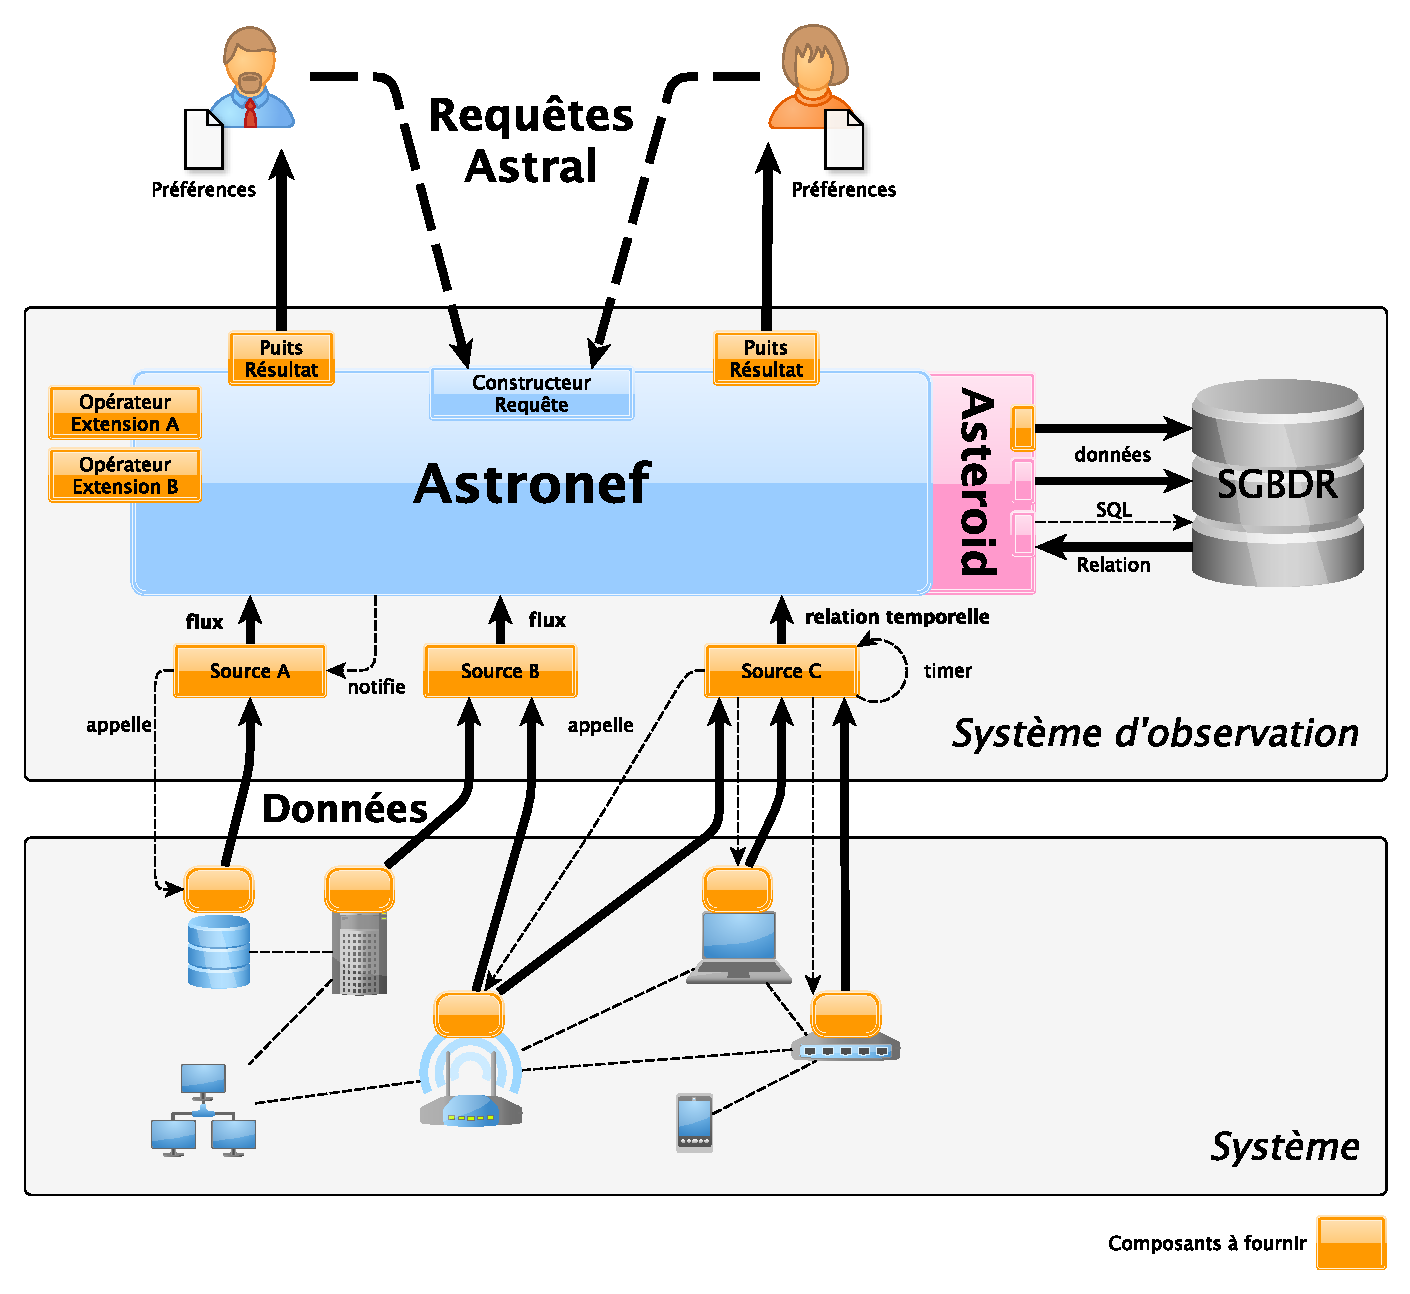
\includegraphics[width=\textwidth]{contrib-global}
	\caption{Présentation des contributions de cette thèse}
\end{figure}
